\documentclass[12pt]{article}

\usepackage{url}
\usepackage{fullpage}
\usepackage{amssymb,amsfonts}
\usepackage{graphicx}

\newcommand{\eps}{\varepsilon}
\newcommand{\R}{\mathbb{R}}

\begin{document}

\thispagestyle{empty}

\begin{center}
{\Large \textsc{CS 125 Algorithms \& Complexity} --- Fall 2016}

\bigskip

{\Large \textsc{Problem Set 2}}

\smallskip

Due: 11:59pm, Friday, September 16th

\bigskip

{\footnotesize See homework submission instructions at \url{http://seas.harvard.edu/~cs125/fall16/schedule.htm}}
\end{center}

\textbf{Problem 5 is worth one-third of this problem set, and problems 1-4 constitute the remaining two-thirds.}

\bigskip

\textbf{When asked to give an algorithm, you should prove correctness and analyze running time unless the problem states otherwise.}

\section*{Problem 1}

You just bought an $m$ gallon (i.e.\ $128m$ ounce) leather bag and want to fill it with spices. You are at your friend's spice shop, and all spices for sale are in powder form. There are $n$ different spices available, and there are $s_i$ ounces of spice $i$ available for each $i=1,\ldots,n$. Each $s_i$ is a positive integer. Furthermore, you know that the market price for spice $i$ is $p_i$ dollars per ounce. Your friend, being the great friend that she is, is willing to let you fill your $128m$ gallon bag with as much of her spices as you wish, {\em for free}! Naturally, you decide to pack the most value you can into your bag that fits. Spices, being in powdered form, can be packed into your bag in any fractional amount. Give an algorithm to decide which spices, and how much of each spice, to pack in your bag. You may assume addition, subtraction and multiplication are constant time operations.

\section*{Problem 2}

There are $n$ horizontal line segments in the plane. The $i$th segment has some height $h_i$ (which may be negative) and runs from $x = a_i to x = b_i$ ($a_i < b_i$). Segments do not contain their endpoints. You must draw a set of vertical lines (note lines and not line segments, and they can be drawn at non-integer coordinates) so that every given horizontal segment is intersected at least once.
\begin{itemize}
\item[(a)] (4 points) Give a greedy algorithm which minimizes the total number of lines drawn and prove its correctness. The running time should be $O(n log n)$.
\item[(b)] (3 points) Suppose the objective was instead to minimize the maximum number of times that any horizontal segment is intersected by vertical lines. That is, each segment should be intersected at least once, and at most $z$ times such that $z$ is minimized. Show that if the optimal solution for a given instance achieves a value of $z_{opt}$ , then there is a greedy solution which is optimal for part (a) while achievng $z \le z_{opt} + 1$ for this new objective.
\item[(c)] (3 points) Assuming that the statement of (b) is true, derive an algorithm which achieves the objective of (b) but with z = $z_{opt}$ . Any algorithm running in polynomial time (i.e.\ $O(n^c)$ for some constant $c>0$) will receive full credit.
\end{itemize}


\section*{Problem 3}

In class we saw that with the disjoint forests data structure, if you use both ``union by rank'' and ``path compression'', a sequence of $n$ make-set and $m\ge n$ find and union operations takes time $O(m\log^* n)$. As you probably noticed, the proof for that bound is non-trivial, which might leave you wondering, could I possibly simplify the data structure and still achieve this bound? Along that train of thought, suppose we use only one of ``union by rank'' or ``path compression'', but not both. Show that if we only use union by rank, there is an infinite family of operation sequences (with $m, n$ going to $\infty$) such that the total runtime to serve a sequence in this family is $\Omega(m\log n)$. Similarly, show that if we only use path compression, we can also make the total time $\Omega(m\log n)$. In both of your example sequences, $m$ should be $\Theta(n)$. \textbf{Hint}: you may find the following {\em sequence} of trees useful to think about:

\begin{center}
\scalebox{.3}{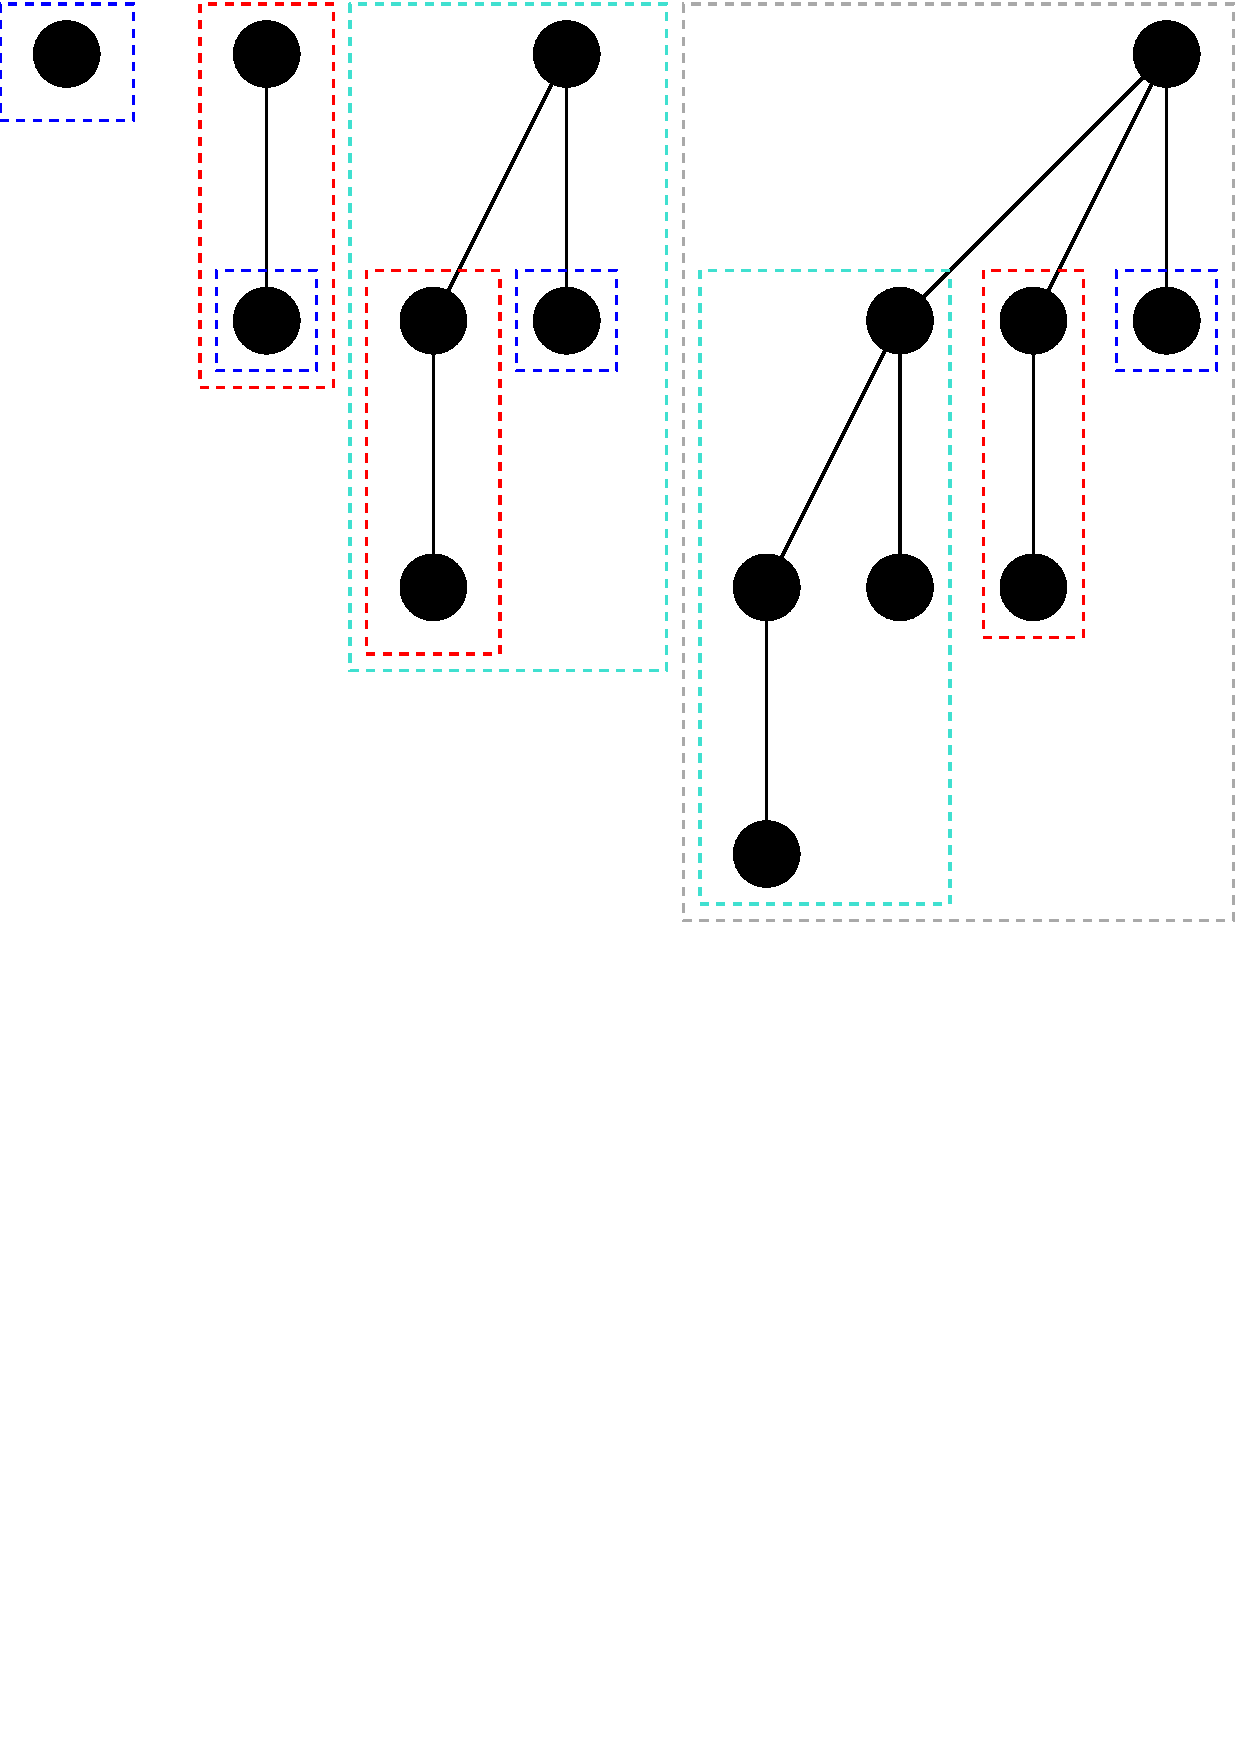
\includegraphics{binomial}}
\end{center}


\section*{Problem 4}
You are given $n$ boxes labeled $1,2,\ldots,n$, each initially in its own stack. You would like a data structure supporting the following two operations:
\begin{itemize}
\item \textbf{move}($x,y$): lift the stack containing box $x$ and place it directly on top opf the stack containing box $y$
\item \textbf{under}($x$): return the number of boxes under $x$ in its stack.
\end{itemize}

Describe a data structure which supports any sequence of $m$ \textbf{move} and \textbf{under} operations efficiently.


\section*{Problem 5 (Programming Problem)}
Solve ``CABLE'' on the programming server \url{https://cs125.seas.harvard.edu}.\\
(under ``Problem Set 2'').

\end{document}